\documentclass{article}

\usepackage{fancyhdr} % Required for custom headers
\usepackage{lastpage} % Required to determine the last page for the footer
\usepackage{extramarks} % Required for headers and footers
\usepackage{graphicx} % Required to insert images
\usepackage{lipsum} % Used for inserting dummy 'Lorem ipsum' text into the template

\usepackage{amsmath}
\usepackage{tikz}
\usetikzlibrary{trees}

% Margins
\topmargin=-0.45in
\evensidemargin=0in
\oddsidemargin=0in
\textwidth=6.5in
\textheight=9.0in
\headsep=0.25in 

\linespread{1.1} % Line spacing

% Set up the header and footer
\pagestyle{fancy}
\lhead{\hmwkAuthorName} % Top left header
\chead{\hmwkClass\ : \hmwkTitle} % Top center header
\rhead{\firstxmark} % Top right header
\lfoot{\lastxmark} % Bottom left footer
\cfoot{} % Bottom center footer
\rfoot{Page\ \thepage\ of\ \pageref{LastPage}} % Bottom right footer
\renewcommand\headrulewidth{0.4pt} % Size of the header rule
\renewcommand\footrulewidth{0.4pt} % Size of the footer rule

\setlength\parindent{0pt} % Removes all indentation from paragraphs

%----------------------------------------------------------------------------------------
%       DOCUMENT STRUCTURE COMMANDS
%       Skip this unless you know what you're doing
%----------------------------------------------------------------------------------------

% Header and footer for when a page split occurs within a problem environment
\newcommand{\enterProblemHeader}[1]{
\nobreak\extramarks{#1}{#1 continued on next page\ldots}\nobreak
\nobreak\extramarks{#1 (continued)}{#1 continued on next page\ldots}\nobreak
}

% Header and footer for when a page split occurs between problem environments
\newcommand{\exitProblemHeader}[1]{
\nobreak\extramarks{#1 (continued)}{#1 continued on next page\ldots}\nobreak
\nobreak\extramarks{#1}{}\nobreak
}

\setcounter{secnumdepth}{0} % Removes default section numbers
\newcounter{homeworkProblemCounter} % Creates a counter to keep track of the number of problems

\newcommand{\homeworkProblemName}{}
\newenvironment{homeworkProblem}[1][Problem \arabic{homeworkProblemCounter}]{ % Makes a new environment called homeworkProblem which takes 1 argument (custom name) but the default is "Problem #"
\stepcounter{homeworkProblemCounter} % Increase counter for number of problems
\renewcommand{\homeworkProblemName}{#1} % Assign \homeworkProblemName the name of the problem
\section{\homeworkProblemName} % Make a section in the document with the custom problem count
\enterProblemHeader{\homeworkProblemName} % Header and footer within the environment
}{
\exitProblemHeader{\homeworkProblemName} % Header and footer after the environment
}

\newcommand{\problemAnswer}[1]{ % Defines the problem answer command with the content as the only argument
\noindent\framebox[\columnwidth][c]{\begin{minipage}{0.98\columnwidth}#1\end{minipage}} % Makes the box around the problem answer and puts the content inside
}

\newcommand{\homeworkSectionName}{}
\newenvironment{homeworkSection}[1]{ % New environment for sections within homework problems, takes 1 argument - the name of the section
\renewcommand{\homeworkSectionName}{#1} % Assign \homeworkSectionName to the name of the section from the environment argument
\subsection{\homeworkSectionName} % Make a subsection with the custom name of the subsection
\enterProblemHeader{\homeworkProblemName\ [\homeworkSectionName]} % Header and footer within the environment
}{
\enterProblemHeader{\homeworkProblemName} % Header and footer after the environment
}
   
%----------------------------------------------------------------------------------------
%       NAME AND CLASS SECTION
%----------------------------------------------------------------------------------------

\newcommand{\hmwkTitle}{Assignment\ \#1 } % Assignment title
\newcommand{\hmwkDueDate}{Tuesday,\ September\ 23,\ 2015} % Due date
\newcommand{\hmwkClass}{CSCI-567} % Course/class
\newcommand{\hmwkClassTime}{} % Class/lecture time
\newcommand{\hmwkAuthorName}{Saket Choudhary} % Your name
\newcommand{\hmwkAuthorID}{2170058637} % Teacher/lecturer
%----------------------------------------------------------------------------------------
%       TITLE PAGE
%----------------------------------------------------------------------------------------

\title{
\vspace{2in}
\textmd{\textbf{\hmwkClass:\ \hmwkTitle}}\\
\normalsize\vspace{0.1in}\small{Due\ on\ \hmwkDueDate}\\
\vspace{0.1in}\large{\textit{\hmwkClassTime}}
\vspace{3in}
}

\author{\textbf{\hmwkAuthorName} \\
        \textbf{\hmwkAuthorID}
        }
\date{} % Insert date here if you want it to appear below your name

%----------------------------------------------------------------------------------------
\tikzstyle{level 1}=[level distance=1.5cm, sibling distance=2.5cm]
\tikzstyle{level 2}=[level distance=1cm, sibling distance=2cm]
\tikzstyle{level 3}=[level distance=1cm, sibling distance=1.5cm]

\begin{document}

\maketitle

%----------------------------------------------------------------------------------------
%       TABLE OF CONTENTS
%----------------------------------------------------------------------------------------

%\setcounter{tocdepth}{1} % Uncomment this line if you don't want subsections listed in the ToC

\newpage
\tableofcontents
\newpage


%----------------------------------------------------------------------------------------
%       PROBLEM 2
%----------------------------------------------------------------------------------------

\begin{homeworkProblem}[Problem \# 1] % Custom section title


\begin{homeworkSection}{\homeworkProblemName:~(a) 1} % Section within problem
%\lipsum[4]\vspace{10pt} % Question

\problemAnswer{ % Answer
Given: $X_i \sim Beta(\alpha, 1)$
MLE for $\alpha$:

Consider $X=(X_1,X_2, \dots, X_n)$
Likelihood function: $L(\alpha|X)$
$L(\alpha | X) = \prod_{i=1}^n f(x_i)$
where
\begin{align}
 f(x_i)&=\frac{\Gamma(\alpha+\beta)}{\Gamma(\alpha)\Gamma(\beta)}x^{\alpha-1}(1-x)^{\beta-1} = \frac{\Gamma(\alpha +1)}{\Gamma(\alpha)\Gamma(1)}x^{\alpha-1}\\
 &=\frac{\alpha \Gamma(\alpha)}{\Gamma(\alpha)} x^{\alpha-1}
 &=\alpha x^{\alpha-1}	
\end{align}

\begin{align}
L(\alpha|X)&=\big(\frac{\Gamma(\alpha+1)}{\Gamma(\alpha)\Gamma(1)}\big)^n \prod_{i=1}^n (x_i)^{\alpha-1}
\end{align}

\begin{align}
LL=\log(L(\alpha | X)) &= n \log(\alpha) + (\alpha -1)\sum_{i=1}^n x_i \\
\frac{dLL}{d\alpha} &= \frac{n}{\alpha} + \sum_{i=1}^n{\log(x_i)}\\
\frac{dLL}{d\alpha} &= 0 \implies \hat{\alpha} =  \frac{n}{\sum_{i=1}^n log(1/x_i)}
\end{align}
Minima at $\hat{\alpha} =  \frac{n}{\sum_{i=1}^n log(1/x_i)}$ is guaranteed due to $\log$ being a concave function.



}




\end{homeworkSection}

%--------------------------------------------

\begin{homeworkSection}{\homeworkProblemName:~(a) 2} % Section within problem
\problemAnswer{ % Answer
Given: $x_i \sim N(\theta, \theta)$ i.e $f(x_i)= (2\pi \theta)^{-\frac{1}{2}} e^{-\frac{(x_i-\theta)^2}{2\theta}}$
MLE estimate for $\theta$:

\begin{align}
L(\theta|X) &=  (2\pi \theta)^{-\frac{N}{2}} e^{-\sum_{i=1}^n\frac{(x_i-\theta)^2}{2\theta}}\\
LL=\log(L(\theta|X)) &= -\frac{N}{2} \log((2\pi \theta)) -\sum_{i=1}^n\frac{(x_i-\theta)^2}{2\theta} \\
\frac{dLL}{d\theta} &= -\frac{N}{2}(\frac{1}{\theta})+\frac{\sum_{i=1}^n x_i^2}{2\theta^2}-\frac{N\theta}{2}\\
\frac{dLL}{d\theta} &=0 \implies N\theta^2+N\theta-\sum_{i=1}^n x_i^2 =0
\end{align}
The above equation is a quadratic and will have two solutions,
Since, $\theta \geq 0$ (a constraint that comes from $\theta$ being the variance), the 

$\theta = \frac{-N\pm \sqrt{N^2+4N\sum_{i=1}^nx_i^2}}{2N}$

Since, $\hat{\theta} \geq 0$, $\hat{\theta} = \frac{-N + \sqrt{N^2+4N\sum_{i=1}^nx_i^2}}{2N}$

}
\end{homeworkSection}

%--------------------------------------------


\begin{homeworkSection}{\homeworkProblemName:~(b) 1} % Using the problem name elsewhere
\problemAnswer{ % Answer
Given: $\hat{f(x)}=\frac{1}{n}\sum_{i=1}^n \frac{1}{h}K(\frac{x-X_i}{h})$
To show: $E_{X_1,X_2, \dots X_n}[\hat{f(x)}]=\frac{1}{h}\int K(\frac{x-t}{h})f(t)dt $

Proof:\\
\begin{align}
E[\hat{f(x)}] &= E[\frac{1}{n}\sum_{i=1}^n \frac{1}{h}K(\frac{x-X_i}{h})]\\
&=\frac{1}{nh}E[K(\frac{x-X_i}{h})]\\
&=\frac{1}{h}E[K(\frac{x-X_1}{h})]
&=\frac{1}{h}E[K(\frac{x-t}{h})]
\end{align}

where the penultimate equality comes from the fact that $X_i$ are iid for all $i \in [1,n]$.
and $t ~ X$%E_{X_1,X_2, \dots X_n}[\hat{f(x)}] = \int \hat{f(x)}f(x)dx

and hence.
\begin{align}
E[\hat{f(x)}]&=\frac{1}{h}E[K(\frac{x-X_1}{h})]
&=\frac{1}{h}\int K(\frac{x-t}{h}) f(t)dt
& = RHS  
\end{align}

}
\end{homeworkSection}

%--------------------------------------------

\begin{homeworkSection}{\homeworkProblemName:~(b) 2}
\problemAnswer{ % Answer
Consider $z = \frac{x-t}{h}$ $\implies$ $t=x-hu$

Then, \begin{align}
E[\hat{f(x)}] &= \frac{1}{h} \int K(z)f(x-hz)dz\\
 \end{align}
 
 $f(x-hz) = f(x) - f'(x)hz + \frac{1}{2}f''(x)\frac{(hz)^2}{2} - \frac{1}{3}f'''(x)\frac{(hz)^3}{3!} + \dots + (-1)^{n}\frac{1}{n!}f^{(n)}(x)(\frac{(hu)^n}{n!})$


By definition, $\int k(z)dz =1$.
Also define an auxilllary variable $M_j=\int k(z)z^j dz$ for the $j^{th}$ moment of the kernel function, 
and hence,
$\int  K(z)f(x-hz)dz=f(x)-hf'(x)M_1+\frac{1}{2}(h^2)f^{''}(x)M_2+\dots+(-1)^n\frac{1}{n!}f^{(n)}M_n$
Now, $Bias = E[\hat{f(x)}]-f(x)=-hf'(x)M_1+\frac{1}{2}(h^2)f^{''}(x)M_2+\dots+(-1)^n\frac{1}{n!}f^{(n)}M_n$

And as $h \longrightarrow 0$, $Bias \longrightarrow 0$
}
\end{homeworkSection}

%--------------------------------------------

\end{homeworkProblem}

%----------------------------------------------------------------------------------------
%       PROBLEM 4
%----------------------------------------------------------------------------------------

\begin{homeworkProblem}[Problem 2] % Roman numerals

\begin{homeworkSection}{\homeworkProblemName:~(a)}
\problemAnswer{

	
		Mean $\bar{x} = \frac{1}{N}\sum x = \frac{1}{10}\sum_{i=1}^{10}x_i = 8.6$
		
		Mean $\bar{y} = \frac{1}{N}\sum y = \frac{1}{10}\sum_{i=1}^{10}y_i = 19.6$
		
		Standard deviation $x_{sd} = \sqrt{\frac{\sum_{i=1}^{10} (x_i-\bar{x})^2}{10-1}} = 21.3269$ 
		
		Standard deviation $y_{sd} = \sqrt{\frac{\sum_{i=1}^{10} (x_i-\bar{x})^2}{10-1}} = 25.1960$ 
		
		Student with unknown major: $(9,18)$: 
		
		Normalised to : $(0.0187, -0.0635)$ 
		
\begin{center}


		 \begin{tabular}{|c|c|c|c|c|c|c|}
			\hline \rule[-2ex]{0pt}{5.5ex} ID & x  & y & $x_n$ & $y_n$ & L1 & L2\\ 
			\hline \rule[-2ex]{0pt}{5.5ex} M1 & 10 & 49 & 0.0623 & 1.107  & \underline{1.2117} & 1.168\\ 
			\hline \rule[-2ex]{0pt}{5.5ex} M2 & -12 & 38 & -0.9163 & 0.6928  & 1.6871 & 1.1998 \\ 
			\hline \rule[-2ex]{0pt}{5.5ex} M3 & -9 & 47 & -0.7829 & 1.0317 & 1.8926 & 1.354 \\ 
			\hline \rule[-2ex]{0pt}{5.5ex} EE1 & 29 & 19 & 0.9074 & -0.0226 & \underline{0.9272} & \underline{0.8904}\\ 
			\hline \rule[-2ex]{0pt}{5.5ex} EE2 & 32 & 31 & 1.0409 & 0.4292 & 1.5125 & \underline{1.1341}\\ 
			\hline \rule[-2ex]{0pt}{5.5ex} EE3 & 37 & 38 & 1.2633 & 0.6928 & 1.9985 & 1.4554\\
			\hline \rule[-2ex]{0pt}{5.5ex} CS1 & 8 & 9 & -0.0267 & -0.3991 & \underline{0.3834} & \underline{0.3418} \\ 
			\hline \rule[-2ex]{0pt}{5.5ex} CS2 & 30 & -28 & 0.9519 & -1.7922 & 2.6661 & 1.9678 \\ 
			\hline \rule[-2ex]{0pt}{5.5ex} CS3 & -18 & -19 & -1.1832 & -1.4534 & 2.5942 & 1.8394 \\ 
			\hline \rule[-2ex]{0pt}{5.5ex} CS4 & -21 & 12 & -1.3167 & -0.2862 & 1.5605 & 1.3535 \\ 
			\hline 
		\end{tabular} 
\end{center}		
	Procedure: We first normalise the data point with unknown major using the mean and standard deviation of the known points, and then calculated the L1 and L2 distances.
	L1 distance between two points $(x_1,y_1)$ and $(x_0,y_0$) is defined as : $L1 = |x_1-x_0| +  |y_1-y_0|$
	
	L2 distance is defined as $L2 = \sqrt{(x_1-x_0)^2 + (y_1-y_0)^2}$
		\textbf{For $L1$}:
		
		\textbf{$K=1$}: For $K=1$ the nearest neighbor is CS1 and hence the unknown sample 'could' be a computer science
		
		\textbf{$K=3$}: For $K=3$ the nearest neighbors are M1, EE1, CS1 and hence there is a 'tie'. Choosing the label of the least distance would again result in CS1 as $CS1 < EE1 <M1$.
		
		\textbf{For $L2$}:
		
		\textbf{$K=1$}: For $K=1$ the nearest neighbor is CS1 and hence the unknown sample 'could' be a computer science
		
		\textbf{$K=3$}: For $K=3$ the nearest neighbors are M1, EE1, EE2. Since two nearest neighbors are from EE, we assign it the unknwon sample to be from Electrical engineering.
		
		\textbf{Comparison} For $K=1$, both $L1$ and $L2$ distance metric give the same results, however for $K=3$, the $L1$ metric yields a tie, since the distances are similar but $L2$ metric being a square quantity of a number smaller than 1 further reduces the distances and .....
		TODO
		
		
		
		
		 
		

			
		
			

		
	}
\end{homeworkSection}


\begin{homeworkSection}{\homeworkProblemName:~(b)}
	\problemAnswer{
		Total points: $N$
		
		Total points with label class $c$: $N_c$
		
		Given: $p(x|Y=c)=\frac{K_c}{N_cV}$ and $\sum K_c=K$
		Class prior: $p(Y=c)=\frac{N_c}{N}$
		
		Unconditional density $p(x)=\sum_c p(x|Y=c)p(Y=c) = \sum_c \frac{K_c}{N_cV} \times \frac{N_c}{N}= \sum_c \frac{K_c}{NV} = \frac{K}{NV}$
		
		Posterior $P(Y=c|x)=\frac{P(x|Y=c)\times P(Y=c)}{ P(x) } = \frac{\frac{K_c}{N_cV} \times \frac{N_c}{N} }{\frac{K}{NV}} =\frac{K_c}{K} $
		
		
	}
\end{homeworkSection}

\end{homeworkProblem}


\begin{homeworkProblem}[Problem 3] % Roman numerals
	
	\begin{homeworkSection}{\homeworkProblemName:~(a)}
		\problemAnswer{
			Information gain $G=H[Y]-H[Y|X]$ where $Y$ is the outcome variable and $X$ is an attribute to be split. 
			In our case $Y$= 'Rains or not' In order to maximise gain for a fixed $Y$ we need to minimise the conditional entropy $H[Y|X]$
			$p_{rain}=\frac{9+5+6+3+7+2+3+1}{80}=frac{36}{80}=0.9$ and hence $p_{no-rain}=0.1$
			\begin{align}
					H[Y]&=-p_{rain}\log(p_rain)-p_{no-rain}\log(p_{no-rain})\\
						&= -(0.9\log_2(0.9)+0.1\log_2(0.1)
			\end{align}
			
			

			
			\textbf{Temperature}

			
			
		}

	\end{homeworkSection}
	
	\begin{homeworkSection}{\homeworkProblemName: ~(b)}
		\problemAnswer{
			By default the rightmost branch correspoonds to the parent condition being a YES[FIX ME]
			
			
			\textbf{a}:
			\begin{center}


					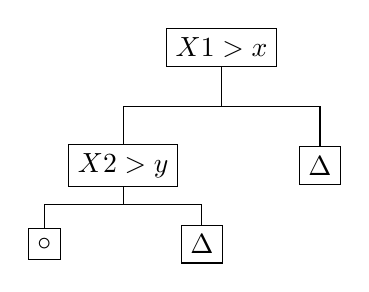
\begin{tikzpicture}
					\tikzstyle{every node}=[draw,rectangle]
					
					\node {$X1>x$}
					[style=edge from parent fork down]

					child {
						node {$X2>y$}
						child { node {$\circ$} }
						child { node {$\Delta$} }
					}
					child { node {$\Delta$} }
					;
					
					\end{tikzpicture}
			\end{center}
					
					
			\textbf{b}:
			\begin{center}
				
				
				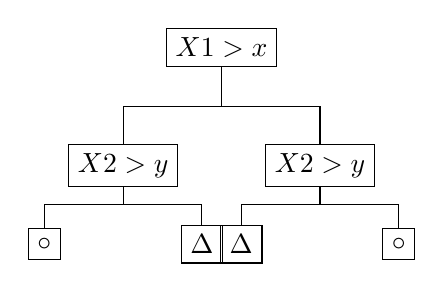
\begin{tikzpicture}
				\tikzstyle{every node}=[draw,rectangle]
				
				\node {$X1>x$}
				[style=edge from parent fork down]
				
				child {
					node {$X2>y$}
					child { node {$\circ$} }
					child { node {$\Delta$} }
				}
				child { 
					node {$X2>y$}
					child { node {$\Delta$} }
					child { node {$\circ$} }
				 }
				;
				
				\end{tikzpicture}
			\end{center}
			
			
				\textbf{c}:
				\begin{center}
					
					
					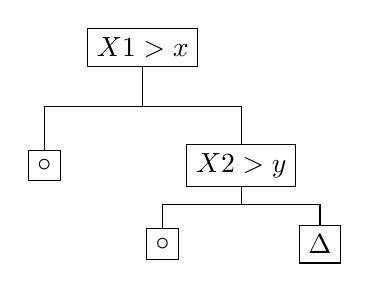
\begin{tikzpicture}
					\tikzstyle{every node}=[draw,rectangle]
					
					\node {$X1>x$}
					[style=edge from parent fork down]
					
					child {
						node {$\circ$}
					}
					child { 
						node {$X2>y$}
						child { node {$\circ$} }
						child { node {$\Delta$} }
					}
					;
					
					\end{tikzpicture}
				\end{center}
				
				
				
				
					\textbf{d}:
					\begin{center}
						
						
						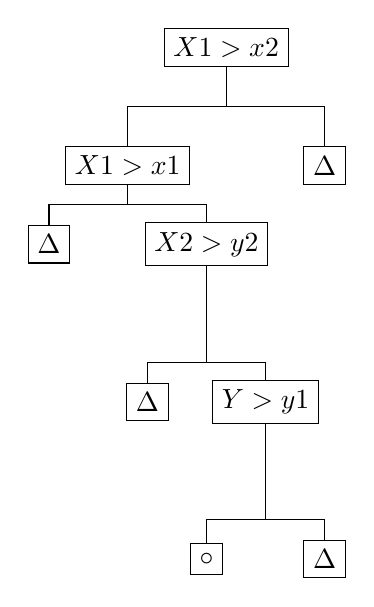
\begin{tikzpicture}
						\tikzstyle{every node}=[draw,rectangle]
						
						\node {$X1>x2$}
						[style=edge from parent fork down]
						
						child { 
							node {$X1>x1$}
							child { node {$\Delta$} }
							child { 
								node {$X2>y2$} 
								child {
									child{node {$\Delta$}}
									child{node {$Y>y1$}
										child{
											child { node {$\circ$} }
											child { node {$\Delta$} }
										}
									}
								}
							}
						}
						child {
							node {$\Delta$}
						}
						;
						
						\end{tikzpicture}
					\end{center}
			
			
			
			}

	\end{homeworkSection}
\end{homeworkProblem}

\begin{homeworkProblem}[Problem 4]
	\begin{homeworkSection}{\homeworkProblemName: ~(a)}
			\problemAnswer{
				 Given a random variable $X \in \mathbf{R}^D$ and $Y \in [C]$ naive bayes defines the joint distribution:
				 \begin{align*}
					P(X=x,Y=y)&=P(Y=y)P(X=x|Y=y)\\
					&=P(Y=y)\prod_{d=1}^D P(X_d=x_d|Y=y)
				 \end{align*}
				 
					Y is a categorical variable with $P(Y=k)=p_k$ for $k \in [1,K]$
					
					Given: $P (x_j |Y=y_k )\sim N(\mu_{jk}, \sigma_{jk})$ $\implies$
					
					\begin{equation}
						\log(P(x_j|Y=k)) = -\frac{\log(2\pi \sigma_{jk})}{2} - \frac{(x_j-x_{jk})^2}{2\sigma_{jk}}
					\end{equation}
					
					

					
					For all $j\neq j'$ $x_j,X_{j'}$ are independent attributes.
					
					Naive bayes: 
					\begin{align*}
						P(X_i=\vec{x},Y_i=y)&=P(Y_i=y)P(X_{i1}=x_1,X_{i2}=x_2\dots X_{iD}=x_D|Y=y_k)\\
						&=P(Y_i=y) \prod_{j=1}^D P(X_{ij}=x_j|Y=y_i)\ \text{Assuming independence of attributes $x_i$}
					\end{align*}
					Each $Y_i$ belongs to one of the $K$ classes, thus $\sum_{k=1}^K p_k=1$ for any $Y_i$
					
					Let $N_k$ represent the number of elements in class $k$ for $k \in [1,K]$
					
					
					Then, $\sum_{i=1}^N \log(Y_i=y_i) = \sum_{k=1}^K P(Y=k) \times N_k $
					
					Consider the likelihood function 
					\begin{align}
						L(\mu,\sigma,p|(X,Y)) &=  \prod_{1}^N P(Y_i=y_i)\times \prod_{j=1}^D P(X_i=x_{ij}|Y=y_i)\\
						\log(L)&= \sum_{i=1}^N \log(P(Y_i=y_i)) +\sum_{i=1}^N \sum_{j=1}^D \log(P(X_i=x_{ij}|Y=y_{i}))\\
						&= \sum_{i=1}^N \log(P(Y_i=y_i)) +\sum_{i=1}^N \sum_{j=1}^D \log(P(X_{ij}=x_{ij}|Y=y_{i}))\\
						&=\sum_{k=1}^K P(Y=k) \times N_k + \sum_{k=1}^K \sum_{j=1}^D \log(P(X_{ij}=x_{ij}|Y=k)) \times N_k
					\end{align}
					
					Now, 
					\begin{align}
					\label{rho1}\frac{\partial{LL}}{\partial{p_k}}&=0\\
					\label{rho2}\frac{\partial{LL}}{\partial{\mu_{jk}}}&=0\\
					\label{rho3}\frac{\partial{LL}}{\partial{\sigma{jk}}}&=0\\
					\end{align}
				}
				\clearpage
				\problemAnswer{
					For for equation \ref{rho1} and constraint $\sum_k p_k =1$, we get: $p_k \frac{N_k}{N}$
					\clearpage
					For equation \ref{rho2},
					\begin{align*}
						\frac{\partial{\sum_{k=1}^K \sum_{j=1}^D \log(P(X_i=x_{ij}|Y=k)) \times N_k}}{\partial \mu_{jk}} &=0\\
						\frac{\sum_{i;Y_i=k}(x_{ij}-\mu_{jk})}{\sigma_{jk}}=0\\
						%-\frac{\sum_{k=1}^KN_k(x_j-\mu_{jk})}{\sigma_{jk}} &=0\\
						\hat{\mu_{jk}} = \frac{\sum_{i;Y_i=k}x_{ij}}{N_k}
					\end{align*}
					
					For equation \ref{rho3},
					\begin{align*}
						\frac{\partial{\sum_{k=1}^K \sum_{j=1}^D \log(P(X_i=x_{ij}|Y=k)) \times N_k}}{\partial \sigma_{jk}} &=0\\
						\frac{\partial}{\partial{\sigma_{jk}}}\sum_{i;Y_i=k}\big(-\frac{\log(2\pi \sigma_{jk})}{2} - \frac{(x_{ij}-x_{jk})^2}{2\sigma_{jk}}\big)=0\\
						\frac{\partial}{\partial{\sigma_{jk}}}\sum_{i;Y_i=k}\big(-\frac{1}{\sigma_{jk}} + \frac{(x_{ij}-x_{jk})^2}{2\sigma_{jk}^2}\big)=0\\
						\hat{\sigma_{jk}}=\frac{\sum_{i;Y_i=k}(x_{ij}-\hat{\mu_{jk}})^2}{N_k}
					\end{align*}
					Constraint $\sum_k p_k =1$
					Given $K$ number of classes, the above constraint the MLE estimate of $p_k$ is given by: $\frac{N_k}{N}$
				}
	\end{homeworkSection}
		\begin{homeworkSection}{\homeworkProblemName: ~(b)}
			\problemAnswer{
				Given: $P(Y=1)=\pi$; For $X_j$ feature, $P(X_j=x_j|Y_k)=\theta_{jk}^{x_j} (1-\theta_{jk})^{1-x_j}$
			\begin{align*}
				P(Y=1|X) &= \frac{P(X|Y=1)P(Y=1)}{P(X)}\\
				 &= \frac{P(X|Y=1)P(Y=1)}{P(X|Y=1)P(Y=1)+P(X|Y=0)P(Y=0)}\\
				 &= \frac{1}{1+\frac{P(X|Y=0)P(Y=0)}{P(X|Y=1)P(Y=1)}}\\
				 &= \frac{1}{1+\exp(\log(\frac{P(X|Y=0)P(Y=0)}{P(X|Y=1)P(Y=1)}))}\\
				 &= \frac{1}{1+\exp(\log({P(X|Y=0)P(Y=0)})-\log({P(X|Y=1)P(Y=1)}))}\\
 				 &= \frac{1}{1+\exp(-(\log(\frac{P(Y=1)}{P(Y=0)}))+\log(P(X|Y=0))-\log(P(X|Y=1)))}\\
			\end{align*}
			
			Now assuming features satisfy the independence property, $P(X|Y=1) = \prod_{j=1}^D P(X_j|Y=1) = \prod_{j=1}^D \theta_{jk}^{x_j} (1-\theta_{jk})^{1-x_j}$
			
			Alternatively,
			
			\begin{align}
			\label{log4b}
				\log(P(X_j|Y=1)) &= \log(\theta_{j1}^{x_j} (1-\theta_{j1})^{1-x_j})\\ 
				&= x_j \log(\theta_{j1}) + (1-x_j)\log((1-\theta_{j1}) \\
				&= x_j  \log(\frac{\theta_{j1}}{1-\theta_{j1}}) + \log(1-\theta_{j1})	
			\end{align}
			
			and,
			
			\begin{align}
		\label{log4c}
		\log(P(X_j|Y=0)) &= \log(\theta_{j0}^{x_j} (1-\theta_{j0})^{1-x_j})\\ 
		&= x_j \log(\theta_{j0}) + (1-x_j)\log((1-\theta_{j0}) \\
		&= x_j  \log(\frac{\theta_{j0}}{1-\theta_{j0}}) + \log(1-\theta_{j0})	
		\end{align}
			
			Hence,
			
			\begin{equation}
			\label{log4b}
			\log(P(X_j|Y=0) - \log(P(X_j|Y=1)) = x_j\log(\frac{\theta_{j0}(1-\theta_{j1})}{\theta_{j1}(1-\theta_{j0})}) + \log\frac{(1-\theta_{j0})}{(1-\theta_{j1})}
			\end{equation}
			
			And hence $\vec{w_j} = \log(\frac{\theta_{j0}(1-\theta_{j1})}{\theta_{j1}(1-\theta_{j0})})$ 	
			
			$w_0= \log(\frac{1-\pi}{\pi} \times (\frac{1-\theta_{j1}}{1-\theta_{j0}})^D)$
		}
		
		\end{homeworkSection}	
\end{homeworkProblem}
%----------------------------------------------------------------------------------------

\end{document}
